% !TEX root = ../notes_template.tex

\chapter{테일러 급수와 로랑 급수}

이 장에서는 영역 $D$에 정의된 복소해석함수 $f$는 
$D$의 임의의 점에서 급수 전개가 가능하다는 근본적인 성질을 먼저 공부할 것이다.
다음 그림에서 왼쪽을 참고하라.
\begin{figure*}[h!]
\begin{center}
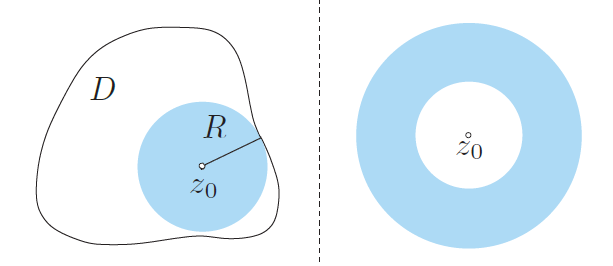
\includegraphics[width=0.5\textwidth]{./SaltChapter/fig-4-0-1}
\end{center}
\end{figure*}
\[
\text{테일러 급수: } \sum_{n=0}^\infty c_n(z-z_0)^n 
\quad
\text{로랑 급수: } \sum_{n\in \mathbb Z} c_n(z-z_0)^n 
\]

즉, 각각의 $z_0 \in D$에 대하여 다음을 만족하는 $R>0$이 존재한다.
\[
f(z) = \sum_{n=0}^\infty c_n(z-z_0)^n, \quad |z-z_0| <R.
\]
역으로,  적당한 $R$에 대하여 $|z-z_0|<R$을 만족하는 두 개 이상의 점에서 급수
\[
\sum_{n=0}^\infty c_n(z-z_0)^n
\]
가 수렴하면 $|z-z_0|<R$에서 복소해석함수이다.
이를 보이는 과정에서 복소해석함수에 대한 근본적인 성질들을 증명할 것이다.
\begin{itemize}
\item[(1)] (일반화된) 코시 적분공식과 코시 부등식
\item[(2)] 해의 분류와 항등정리
\item[(3)] 최대절대값정리
\end{itemize}

이 장의 후반부에서는
급수와 유사하지만 $z-z_0$ 항의 지수를 음의 정수까지 확장한
로랑 급수를 공부할 것이다.
이는 원환(특히 뚫린 원판)에 정의된 복소해석함수를 연구하는데 특히 유용하다,
앞의 그림에서 오른쪽을 참고하라.
끝으로 로랑 급수는 ``특이점''의 분류와 실함수 적분의 계산에도 유용함을 살펴볼 것이다.

\section{급수}

실수열의 경우와 유사하게 주어진
복소수열 $(a_n)_{n\in\mathbb N}$에 대하여
부분합 수열 $(s_n)_{n\in\mathbb N}$을 만들 수 있다.
\begin{align*}
s_1 &:= a_1, \\
s_2 &:= a_1 + a_2, \\
s_3 &:= a_1 + a_2 + a_3, \\
& \vdots
\end{align*}

\begin{salt_definition} \label{def-4-1}
\
\begin{itemize}
\item[(1)] 복소수열 $(s_n)_{n\in\mathbb N}$이 수렴하면
$\sum\limits_{n=1}^\infty a_n := \lim\limits_{n\to\infty} s_n$라 쓰고
급수 $\sum\limits_{n=1}^\infty a_n$이 {\bf 수렴한다}고 정의한다.
\item[(2)] 복소수열 $(s_n)_{n\in\mathbb N}$이 발산하면,
급수 $\sum\limits_{n=1}^\infty a_n$는 {\bf 발산한다}고 정의한다.
\item[(3)] 실급수 $\sum\limits_{n=1}^\infty |a_n|$이 수렴하면,
급수 $\sum\limits_{n=1}^\infty a_n$은 {\bf 절대수렴한다}고 정의한다.
\end{itemize}
\end{salt_definition}

복소수열이 수렴할 필요충분조건은
실수부와 허수부로 만든 수열이 각각 수렴하는 것이라는 
연습문제 \ref{ex-1-25}의 결과로부터,
\[
\sum\limits_{n=1}^\infty a_n\,\text{이 수렴한다. }
\Longleftrightarrow \text{\textcolor{red}{ 실수열} }
\sum\limits_{n=1}^\infty \Re(a_n)\, \text{과 }
\sum\limits_{n=1}^\infty \Im(a_n)\,\text{가 수렴한다.}
\]
따라서  실해석학의 결과를 아용하여 복소수열의 수렴성을 판정할 수 있다.
예를 들면, 다음 결과들을 쉽게 얻을 수 있는데 이는 연습문제로 남긴다.

\begin{salt_exercise}\label{ex-4-1}
$\Sum_{n=1}^\infty a_n$이 수렴하면, $\Lim_{n\to\infty}a_n = 0$임을 보여라.
\end{salt_exercise}

\begin{salt_exercise}\label{ex-4-2}
$\Sum_{n=1}^\infty a_n$이 절대수렴하면, $\Sum_{n=1}^\infty a_n$이 수렴함을 증명하라.
\end{salt_exercise}

\begin{salt_exercise}\label{ex-4-3}
$|z|<1$이면 $\Sum_{n=0}^\infty z^n$이 수렴하고 
$\Sum_{n=0}^\infty z^n = \dfrac1{1-z}$임을 보여라.
\end{salt_exercise}

\begin{salt_exercise}\label{ex-4-4}
$|z|<1$이면 $\Sum_{n=0}^\infty nz^{(n-1)^2}$임을 보여라.
\end{salt_exercise}

\begin{salt_exercise}\label{ex-4-5}
$\Re(s)>0$인 모든 복소수 $s\in \mathbb C$에 대하여
$1^{-s} +  2^{-s} + 3^{-s} + \cdots$가 수렴함을 보여라.
그러면
\[
s \mapsto \zeta(s) := \sum_{n=1}^\infty \dfrac1{n^s}
\]
\end{salt_exercise}
는 반평면 $\Re(s)>1$에서 잘 정의된 함수가 되며, 이를 
{\bf 리만 제타함수}라고 한다.
리만 제타함수와 정수론의 소수이론을 연결한 {\bf 오일러 곱셈공식}에 따르면,
소수를 증가하는 순서대로 나열한
$p_1:=2 < p_2:=3 < p_3:=5 < \cdots$를 무한 소수열로 정의할 때 다음이 성립한다.
\[
\zeta(s) = \lim_{K\to \infty} \prod_{k=1}^K \dfrac1{1-p_k^{-s}},
\quad \Re(s)>1.
\]
버나드 리만(1826-1866)은 제타함수 $\zeta$를 확장하여 $\mathbb C\setminus \{1\}$의 
복소해석함수로 정의할 수 있음을 보였다. 
$\zeta$는 $-2, -4, -6, \ldots$에서 ``자명해(trivial zero)''를 갖지면
다른 해도 존재한다. 리만이 계산한 모든 비자명해(nontrivial zero)는 모두 직선 $\Re(s) = 1/2$위에
있다. 이로부터 리만은 다음과 같이 예측(conjecture)하였는데 이는 여전히 수학계의 유명한 미해결 문제이다.

\begin{salt_conjecture}[리만가설] \label{conj-4-1}
리만 제타함수의 모든 비자명해는 직선 $\Re(s) = 1/2$ 위에 있다.
\end{salt_conjecture}

\section{급수}

\subsection{제곱급수와 수렴영역}

$(c_n)_{n\in\mathbb N}$을 복소수열이라고 하자.
다음과 같은 표현을
\[
\sum_{n=0}^\infty c_nz^n
\]
복소수 변수 $z$의 제곱급수라고 한다 ($(c_n)_{n\in\mathbb N}$을 계수들의 수열로 생각해도 된다).
이제 특정한 값을 급수의  $z$에 대입하는 경우를 생각해볼 수 있다.
그러면 어떤 $z\in\mathbb C$에 대하여 제곱급수가 수렴할 수 있고, 
다른 값에서는 발산할 수도 있다.

\begin{salt_example}\label{example-4-1}
모든 다항식은 유한개의 항에서만 계수가 $0$이 아닌 제곱급수 꼴로 쓸 수 있다.
따라서 다항식은 모든 $z\in\mathbb C$에 대하여 수렴한다.

제곱급수  
\[
\sum_{n=0}^\infty z^n
\]
는 $|z|<1$에서 수렴한다. 
$|z|\ge1$에서 급수는 발산한다 (왜냐하면 $\Lim_{n\to\infty} z^n = 0$이 성립하지 않으므로).
\hfill$\diamondsuit$
\end{salt_example}

근본적인 질문으로 
\begin{center}
어떤 $z\in\mathbb C$에 대하여  급수 $\sum_{n=0}^\infty c_nz^n$가 수렴하는가?
\end{center}

이 문제에 대한 답은 다음 정리에서 얻을 수 있다.

\begin{salt_theorem} \label{thm-4-1}
제곱급수 $\Sum_{n=0}^\infty c_nz^n$에 대하여
다음 두 가지 중 정확히 하나만 성립한다.
\begin{itemize}
\item[(1)] 모든 $z\in\mathbb C$에 대하여 절대수렴하거나
\item[(2)] 음이 아닌 실수 $R$이 유일하게 존재하여 다음을 만족한다.
\begin{itemize}
\item[(a)] $|z|<R$인 모든 $z\in\mathbb C$에 대하여 $\Sum_{n=0}^\infty c_nz^n$이 절대수렴하고,
\item[(b)] $|z|>R$인 모든 $z\in\mathbb C$에 대하여 $\Sum_{n=0}^\infty c_nz^n$는 발산한다.
\end{itemize}
\end{itemize}
\end{salt_theorem}

위 정리에서 유일한 $R>0$을 급수의 수렴반경이라 부른다.
급수가 모든 $z\in\mathbb C$에 대하여 수렴하면
무한대의 수렴반경을 가지며 ``$R=\infty$''라 쓴다.

\begin{figure}[h!]
\begin{center}
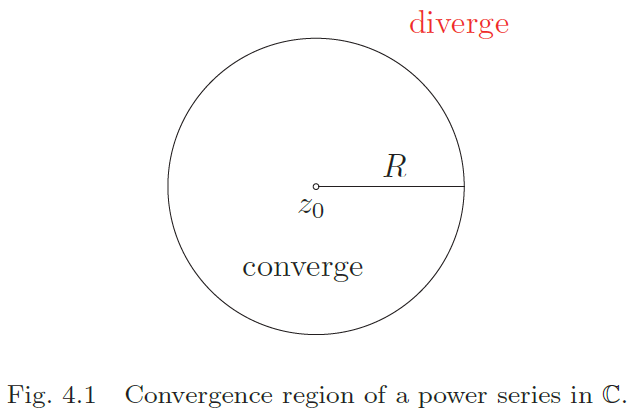
\includegraphics[width=0.5\textwidth]{./SaltChapter/fig-4-1}
\end{center}
\caption{$\mathbb C$에 정의된 제곱급수의 수렴영역}
\label{fig-4-1}
\end{figure}

원 $|z|=R$에서는 어떻게 될까?
복소 제곱급수는 $|z|=R$로 주어진 경계의 모든 점에서 발산하거나,
어떤 점에서는 발산하고 어떤 점에서는 수렴하거나,
아니면 경계의 모든 점에서 수렴할 수도 있다.
경계위의 각 점에 대하여 어떻게 되는지 답을 구하는 일반적인 방법은 없다.
특정한 제곱급수가 주어지면 그 특성에 따라 찾아 직접 확인해야 한다,

{\bf 증명} (정리 \ref{thm-4-1})

\[
S:= \left\{ y\in [0,\infty) \,:\,
\exists z\in \mathbb C, y=|z| \text{ 이고 } \Sum_{n=0}^\infty c_nz^n \text{이 수렴한다.}
\right\}
\]
라 정의하자.
$0\in S$은 분명하기에 $S$는 공집합이 아니며
다음 두 가지 경우가 가능하다.

$\underline{1}^\circ$ $S$가 위로 유계가 아닌 경우:
이 경우는 수렴반경은 무한대가 됨을 보일 것이다.
$z\in \mathbb C$가 주어졌다고 하면,
$|z|<y$인 $y\in S$가 존재한다.
 그런데 $y\in S$이므로 $y=|z_0|$이고
\[
\sum_{n=0}^\infty c_n z_0^n
\]
이 수렴하는 $z_0\in S$가 존재한다.
이로부터 $n\to\infty$일 때 각 항이 $0$으로 수렴한다.
특히, 각 항은  $|c_nz_0^n| \le M$으로 유계이다.
이제 $r:=|z|/|z_0| (<1)$로 잡으면
\[
|c_nz^n| = |c_nz_0^n| \left( \dfrac{|z|}{|z_0|}\right)^n
\le Mr^n \quad (n\in \mathbb N).
\]
한편 $\sum\limits_{n=0}^\infty Mr^n$이 수렴한다 ($r<1$).
비교판정법을 쓰면 
\[
\sum_{n=0}^\infty c_n z^n
\]
은 절대수렴한다. $z$는 우리가 임의로 선택할 수 있기 때문에
정리의 (1)이 성립한다,


$\underline{2}^\circ$ $S$가 위로 유계인 경우:
이 경우 수렴반경이 $\sup S$가 됨을 보일 것이다.
즉,
\begin{itemize}
\item[(a)] $|z|<\sup S$이면
$\Sum_{n=0}^\infty c_nz^n$이 절대수렴하고,
\item[(b)] $|z|>\sup S$이면  $\Sum_{n=0}^\infty c_nz^n$는 발산한다.
\end{itemize}
$z\in S$가 $|z|<\sup S$를 만족하면
상계(supremum)의 %= ##[SALT] 용어확인
정의에 따라,
$|z|<y$인 $y\in S$가 존재한다. 
그러면 $\underline{1}^\circ$ $S$의 증명과정을 아래와 같이 반복할 수 있다.
$y\in S$이므로
$y=|z_0|$이고
\[
\sum_{n=0}^\infty c_n z_0^n
\]
이 수렴하는 $z_0\in S$가 존재한다.
이로부터 $n\to\infty$일 때 각 항이 $0$으로 수렴한다.
특히, 각 항은 $|c_nz_0^n| \le M$으로 유계이다.
이제 $r:=|z|/|z_0| (<1)$로 잡으면
\[
|c_nz^n| = |c_nz_0^n| \left( \dfrac{|z|}{|z_0|}\right)^n
\le Mr^n \quad (n\in \mathbb N).
\]
한편 $\sum\limits_{n=0}^\infty Mr^n$이 수렴한다 ($r<1$).
비교판정법을 쓰면 
\[
\sum_{n=0}^\infty c_n z^n
\]
은 절대수렴한다.
끝으로, $z\in \mathbb C$가 $|z|>\sup S$를 만족하면,
$y:=|z|$라 할 때
$y \in S$이고 $S$의 정의로부터 
\[
\sum_{n=0}^\infty c_n z^n
\]
이 발산한다 (그렇지 않다면 $y\in S$를 만족해야 한다).

\begin{figure*}[h!]
\begin{center}
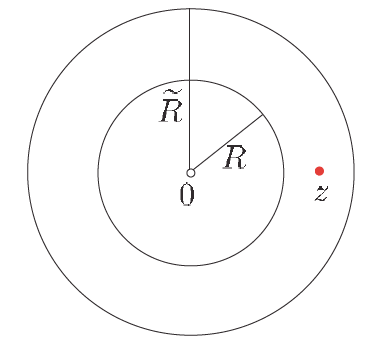
\includegraphics[width=0.3\textwidth]{./SaltChapter/fig-4-0-2}
\end{center}
%\caption{$\mathbb C$에 정의된 제곱급수의 수렴영역}
%\label{fig-4-1}
\end{figure*}

$R$의 유일성은 다음과 같이 증명된다.
$R$과 $\tilde R$이 정리의 조건을 만족하고 $R<\tilde R$이라 하자.
그러면
\[
R < r:= \dfrac{R+\tilde R}{2} < \tilde R.
\]
$r<\tilde R$로부터
$\Sum_{n=0}^\infty c_n r^n$이 수렴하고,
$R<r$로부터 $\Sum_{n=0}^\infty c_n r^n$은 발산하며
모순이 된다.
\hfill $\square$

다음 결과를 이용하면
몇가지 경우의 수렴반경를 계산할 수 있다,

 \begin{salt_theorem} \label{thm-4-2}
제곱급수 
\[
\Sum_{n=0}^\infty c_nz^n
\]에 대하여 극한
$L:= \Lim_{n\to\infty} \left| \dfrac{c_{n+1}}{c_n}\right|$가
존재한다고 하자. 
\begin{itemize}
\item[(1)] $L\ne0$이면, 수렴반경은 $1/L$이고,
\item[(2)] $L=0$이면, 수렴반경은 무한대이다.
\end{itemize}
\end{salt_theorem}

{\bf 증명}

$L\ne0$이라 하자.
그러면 $|z|<1/L$인 모든 $z\ne0$에 대하여
$q<1$와 충분히 큰 $N$이 존재하여
\[
\dfrac{|c_{n+1}z^{n+1}|}{|c_nz^n|}
= \left| \dfrac{c_{n+1}}{c_n}\right| |z| \le q <1
\quad (n>N)
\]
을 만족한다
(왜냐하면,
\[
\left|\dfrac{c_{n+1}}{c_n}z\right|
\stackrel{n\to\infty}{\longrightarrow}
L|z|<1
\]
이므로 $q=(L|z|+1)/2 <1$로 잡으면 된다).
비율판정법을 적용하면 급수는 절대수렴한다.

$L=0$이면 $0$이 아닌 모든 $z\in \mathbb C$에 대하여
$q<1$가 존재하여
\[
\dfrac{|c_{n+1}z^{n+1}|}{|c_nz^n|}
= \left| \dfrac{c_{n+1}}{c_n}\right| |z| \le q <1
\quad (n>N)
\]
을 만족한다 (왜냐하면
\[
\left|\dfrac{c_{n+1}}{c_n}z\right|
\stackrel{n\to\infty}{\longrightarrow}
0|z|=0<1
\]
이므로 $q=1/2<1$도 두면된다).
따라서 비율판정법을 다시 쓰면 급수는 절대수렴한다.

한편, $L\ne0$이고 $|z|>1/L$이면,
$\left|\dfrac{c_{n+1}z}{c_n}\right|
\stackrel{n\to\infty}{\longrightarrow}
L|z|>1$이므로
충분히 큰 $N$이 존재하여
\[
\dfrac{|c_{n+1}z^{n+1}|}{|c_nz^n|}
= \left| \dfrac{c_{n+1}}{c_n}\right| |z|>1
\quad (n>N)
\]
을 만족한다.
이 경우 비율판정법에 따라 급수는 발산한다.
\hfill $\square$

\begin{salt_example}\label{example-4-2}
\[
\lim_{n\to\infty} \dfrac{\dfrac1{(n+1)^2}}{\dfrac1{n^2}} = 1
\]
이므로 
급수 $\Sum_{n=1}^\infty \dfrac{z^n}{n^2}$는
$|z|<1$에서 수렴하고
$|z|>1$에서 발산한다.
$|z|=1$이면
\[
\left| \dfrac{z^n}{n^2} \right| = \dfrac1{n^2}
\]
이므로 급수 $\Sum_{n=1}^\infty \dfrac{1}{n^2}$는
절대수렴한다. 즉, 원 $|z|=1$ 위의 모든 점에서 급수가 수렴한다.
한편 기하급수 
\[
\sum_{n=0}^\infty z^n
\]
은 원 $|z|=1$ 위의 어떤 점에서도 수렴하지 않는다.
\hfill$\diamondsuit$
\end{salt_example}

\begin{salt_exercise}\label{ex-4-6}
급수 $\Sum_{n=0}^\infty c_nz^n$에 대하여
극한 $L:=\Lim_{n\to\infty} sqrt[n]{|c_n|}$이 존재할 때
다음을 보여라.
\begin{itemize}
\item[(1)] $L\ne 0$이면 수렴반경은 $1/L$이다.
\item[(2)] $L\ne0$이면 수렴반경은 무한대이다.
\end{itemize}
\end{salt_exercise}

\begin{salt_exercise}\label{ex-4-7}
급수 $\Sum_{n=1}^\infty n^nz^n$은
$z=0$에서만 수렴함을 보여라.
\end{salt_exercise}

\begin{salt_exercise}\label{ex-4-8}
급수 $\Sum_{n=1}^\infty \dfrac{z^n}{n^n}$은
모든 $z\in\mathbb C$에 대하여 수렴함을 보여라.
\end{salt_exercise}

\begin{salt_exercise}\label{ex-4-9}
다음 복소제곱급수의 수렴반경을 구하라.
\[
\sum_{n=1}^\infty \dfrac{(-1)^n}{n}z^n,\quad
\sum_{n=0}^\infty n^{2012}z^n, \quad
\sum_{n=0}^\infty \dfrac1{n!}z^n.
\]
\end{salt_exercise}

\subsection{복소해석함수의 제곱급수}

다항식은 수렴반경이 무한대인 제곱급수로 간주할 수 있다.
즉, 모든 $\mathbb C$에서 수렴한다.
이 성질은 복소해석함수에서도 성립하는데
이는 우연이 아니다.
일반적으로 제곱급수 
\[
f(z):= \sum_{n=0}^\infty c_nz^n
\]
가 $|z|<R$에 대하여 수렴하면
$|z|<R$에서 복소해석함수가 되며 
다음 등식이 성립한다.
\[
f'(z) = \dfrac d{dz} (c_0+ c_1z + c_2z^2 + \cdots)
= c_1 + 2c_2z + 3c_3z^3 + \cdots 
= \sum_{n=1}^\infty c_n n z^{n-1}.
\]
(항의 개수가 유한한 경우, 즉, 다항식처럼 
항별 미분이 가능할 것으로 예상한 결과와 같다)

\begin{salt_theorem}\label{thm-4-3}
$R>0$이고 $f(z):= \Sum_{n=0}^\infty c_nz^n$가
$|z|<R$에서 수렴한다고 하면
$f'(z) = \Sum_{n=1}^\infty c_n n z^{n-1}$.
\end{salt_theorem}

{\bf 증명}

{\bf 단계 1.}
우선 다음 제곱급수가 $|z|<R$에서 절대수렴함을 보이자.
\[
g(z):= \Sum_{n=1}^\infty c_n n z^{n-1}
=  c_1 + 2c_2z + 3c_3z^3 + \cdots
\]
$z$는 고정하자.
$|z|<r<R$을 만족하는 $r$을 잡으면, 가정으로부터
\[
\Sum_{n=0}^\infty c_nr^n
\]
이 수렴한다. 따라서 모든 $n$에 대하여
$|c_nr^n|<M$을 만족하는 양수 $M$이 존재한다.
$\rho:=|z|/r$이라 하면, $0\le \rho <1$이고,
\[
|nc_nz^{n-1}| = |c_nr^n| \cdot 
\dfrac1r \cdot n \left| \dfrac zr\right|^{n-1}
\le \dfrac{Mn\rho{n-1}}r.
\]
$\Sum_{n=1}^\infty n\rho^{n-1}$은 
($1/(1-\rho)^2$으로) 수렴한다 (연습문제 \ref{ex-4-4} 참고).
따라서 비교판정법에 의해
$\Sum_{n=1}^\infty nc_nz^{n-1}$은 절대수렴한다.

{\bf 단계 2.}
이제 $|z_0|<R$에 대하여 $f'(z_0) = g(z_0)$임을 보이자. 즉,
\[
\lim_{z\to z_0} \left(
\dfrac{f(z)-f(z_0)}{z-z_0} - g(z_0) \right) = 0.
\]
단계 1에서 했던 것처럼 $|z_0|<r<R$을 만족하는 $r$을 잡으면, 
$z\to z_0$로부터 $|z|<r$도 성립한다.

\begin{figure*}[h!]
\begin{center}
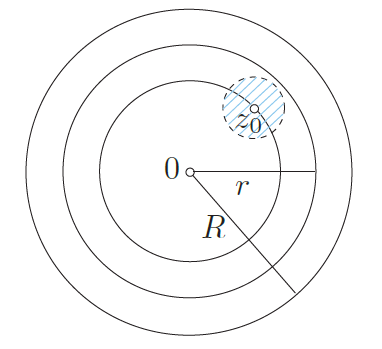
\includegraphics[width=0.3\textwidth]{./SaltChapter/fig-4-0-3}
\end{center}
%\caption{$\mathbb C$에 정의된 제곱급수의 수렴영역}
%\label{fig-4-0-3}
\end{figure*}

$\epsilon>0$이라 하자.
$\Sum_{n=1}^\infty nc_nr^{n-1}$이 절대수렴하므로
다음을 만족하는 $N$이 존재한다.
\[
\Sum_{n=N}^\infty \left| nc_nr^{n-1}\right| < \dfrac \epsilon4.
\]
이제부터 $N$을 고정하자.
$f(z) - f(z_0) = \Sum_{n=1}^\infty c_n(z^n - z_0^n)$이므로,
$z\ne z_0$에 대하여
\[
\dfrac{f(z)-f(z_0)}{z-z_0}  
= \sum_{n=1}^\infty c_n \dfrac{z^n-z_0^n}{z-z_0}
= \sum_{n=1}^\infty c_n \left(
z^{n-1} + z^{n-2}z_0 + \cdots + z_0^{n-1} \right).
\]
따라서,
\[
\dfrac{f(z)-f(z_0)}{z-z_0}   - g(z_0)
= \sum_{n=1}^\infty c_n \dfrac{z^n-z_0^n}{z-z_0}
= \sum_{n=1}^\infty c_n \left(
z^{n-1} + z^{n-2}z_0 + \cdots + z_0^{n-1} - nz_0^{n-1}\right).
\]
이 급수에서 처음 $N-1$개 항의 합을 $S_1$이라 하고
(즉, $n=1$에서 $n=N-1$까지),
$S_2$를 나머지 항의 합이라고 하자.
그러면, $|z|, |z_0| < r$로부터
\[
|S_2| \le \sum_{n=N}^\infty |c_n| 
\left( \underbrace{r^{n-1}+r^{n-1} + \cdots + r^{n-1}}_{n\text{개 항}}
+ nr^{n-1}\right)
= \sum_{n=N}^\infty 2n|c_n|r^{n-1} < \dfrac\epsilon2.
\]
한편,
\[
S_1= \sum_{n=1}^N c_n \left(
z^{n-1} + z^{n-2}z_0 + \cdots + zz_0^{n-2} + z_0^{n-1} - nz_0^{n-1}
\right)
\]
는 $z$의 다항식이며 극한은 다음과 같다.
\begin{align*}
\lim_{z\to z_0} S_1
&= \sum_{n=1}^N c_n \left(
z^{n-1} + z^{n-2}z_0 + \cdots + zz_0^{n-2} + z_0^{n-1} - nz_0^{n-1}
\right) \\
&= \sum_{n=1}^N c_n \left(
nz_0^{n-1}  - nz_0^{n-1} \right) = 0.
\end{align*}
따라서
$|z-z_0|<\delta$이면, $|S_1|< \epsilon/2$가 되는 
양수 $\delta$가 존재한다.
이제 $|z|<r$이고 $0<|z-z_0|< \delta$에 대하여
\[
\left| \dfrac{f(z)-f(z_0)}{z-z_0}   - g(z_0) \right|
\le |S_1| + |S_2| <  \dfrac\epsilon2 + \dfrac\epsilon2 = \epsilon.
\]
이로써 $f'(z_0) = g(z_0)$가 증명된다.
\hfill $\square$

\begin{salt_remark} \label{rem-4-1}
$(c_n)_{n\in\mathbb N}$이 실수열일 때,
실제곱급수
\[
\sum_{n=0}^\infty c_nx^n
\]
\end{salt_remark}
를 생각해보자. 실해석의 결과로부터 어떤 $R>0$이 존재하여
이 제곱급수는 구간 $(-R, R)$에서 수렴하고
$\mathbb R \setminus [-R,R]$에서 발산한다.
정리 \ref{thm-4-1}과 \ref{thm-4-3}로부터
실변수 $x$를 복소변수 $z$로 바꾸면 실제곱급수의 결과가 
복소평면의 원판 $|z|<R$에 정의된 복소해석함수로 확장됨을 알 수 있다.
따라서
실해석함수(즉, 국소적으로 제곱급수 전개를 갖는 실변수함수)는
복소해석함수를 실수축에 제한한 것으로 볼 수 있다.
이 결과로 실해석학과 복소해석학의 세계를 연결하는
상호작용을 엿볼 수 있다
(우리는 이미 앞에서 코시-리만 방정식을 공부하면서 이러한 사례를 살펴 본 바 있다).











